\documentclass[conference]{IEEEtran}
\IEEEoverridecommandlockouts
% The preceding line is only needed to identify funding in the first footnote. If that is unneeded, please comment it out.
\usepackage{cite}
\usepackage{amsmath,amssymb,amsfonts}
\usepackage{algorithmic}
\usepackage{graphicx}
\usepackage{textcomp}
\usepackage{xcolor}
\def\BibTeX{{\rm B\kern-.05em{\sc i\kern-.025em b}\kern-.08em
    T\kern-.1667em\lower.7ex\hbox{E}\kern-.125emX}}
\begin{document}

\title{Scaling up CEG4N framework for State-of-art Neural Networks Architecture\\
%{\footnotesize \textsuperscript{*}Note: Sub-titles are not captured in Xplore and
%should not be used}
\thanks{Identify applicable funding agency here. If none, delete this.}
}


\author{\IEEEauthorblockN{1\textsuperscript{st} Joao Victor Lima de Souza}
\IEEEauthorblockA{\textit{Departamento de Engenharia Elétrica} \\
\textit{Universidade Federal do Amazoans)}\\
Manaus, Amazonas \\
souza.joao@ufam.edu.br}
}

\maketitle

\begin{abstract}

Embedded devices play a crucial role in the functioning of cars, home appliances, medical devices, interactive kiosks, and other equipment we use in our daily lives \cite{c2}. With the ever-growing use of Artificial Intelligence (AI) across a broad spectrum of applications, finding better ways to port these classification methods has become more important than ever.

In our project, we will address the challenge of porting neural networks to smaller systems, such as embedded devices. One way to achieve this is through the process of neural network quantization. However, this method has some drawbacks, such as a loss of accuracy, which may lead to potential vulnerabilities. Our goal is to mitigate these issues and ensure the efficient and secure implementation of AI on embedded systems.
\end{abstract}

\begin{IEEEkeywords}
SMT, QNN, Interval Analysis 
\end{IEEEkeywords}

\section{Introduction}

Embedded devices play a crucial role in the functioning of cars, home appliances, medical devices, interactive kiosks, and other equipment we use in our daily lives\cite{c2}. With the ever-growing use of Artificial Intelligence (AI) across a broad spectrum of applications, finding better ways to port these classification methods has become more important than ever.

In our project, we will address the challenge of porting neural networks to smaller systems, such as embedded devices. One way to achieve this is through the process of neural network quantization. However, this method has some drawbacks, such as a loss of accuracy, which may lead to potential vulnerabilities. Our goal is to mitigate these issues and ensure the efficient and secure implementation of AI on embedded systems.

\section{Context}

The implementation of neural networks in embedded systems is challenged by the computational resource limitations of these devices. Neural networks, due to their intensive computational demands, often exceed the processing capabilities offered by embedded systems. To address this issue, the process of quantization is employed \cite{bnn_overview}, which involves adopting fixed-point representation as opposed to the conventional use of floating-point numbers.

However, it is important to note that quantization leads to a loss of precision in the neural network \cite{c4}, which can have significant implications depending on the application. In the context of this study, maintaining accuracy is of vital importance.

CEG4N \cite{1} is a framework designed to optimize the quantization of neural networks. It employs an SMT solver to identify counter-examples arising during the quantization process. These counter-examples are then leveraged by a genetic algorithm to generate an optimal set of quantization variables.

However, the CEG4N method encounters scalability limitations, particularly with larger neural network models, due to verification algorithms that do not scale effectively for extensive networks.

\section{Objective}
For our project, we will focus on the CEG4N framework. As previously mentioned, this framework has been developed to quantize a neural network and generate an optimal Quantized Neural Network (QNN). However, it has been identified that the current framework is not capable of handling state-of-the-art Artificial Neural Networks (ANNs) due to scalability issues.

Therefore, the primary objective of this work is to enhance the scalability of the CEG4N framework. To achieve this, we will undertake the following approach:
\begin{itemize}
    \item Conduct a comprehensive review of the literature regarding the application of SMT solvers in quantization problems to enhance understanding and identify best practices.
    \item Enhance the scalability of the CEG4N framework by addressing limitations encountered, particularly with larger neural network models.
    \item Investigate the literature on Interval Analysis to identify methods and techniques that can be integrated into the framework to further improve scalability.
    \item Explore the utilization of different solvers available within ESBMC to optimize the scalability of CEG4N, assessing their effectiveness and potential advantages for handling larger neural network models.
\end{itemize}


\section{Background}

\subsection{ANN - \textit{Artificial Neural Net}}
Artificial Neural Networks (ANNs) are mathematical models used for data classification. The essence of their functionality lies in the need to be properly trained to perform this task. During the training process, a collection of data is used, with certain sets serving as inputs and others corresponding to the desired outputs. The underlying purpose is to establish associations between the inputs and outputs, thereby guiding the adjustment of the network's internal parameters.

Through this iterative training process, the neural network gradually assimilates the intrinsic relationships between the input data and the desired outcomes, culminating in the development of a model capable of making classifications based on the learned information. In summary, the training process enables the neural network to discern relevant patterns and relationships, conferring the ability to make accurate classifications on previously unseen data \cite{state-art-ann}.

\subsection{QNN - \textit{Quantized Neural Net}}
Quantized Neural Networks are ANNs with their weights represented by fixed points, i.e., binary or integer values \cite{bnn_overview}. This significantly reduces the computational power required to train the model; however, there is a trade-off in the reduction of the model's accuracy.

Given this decrease in accuracy, our approach aims to test verification methods to identify failures in the tested properties. This will allow us to better understand the challenges arising from quantization and thus seek solutions to mitigate any negative impacts on the quantization process. The intention is to perform these tests on the code implemented in C, aiming for a more comprehensive understanding of the performance of the quantized neural network and enabling improvements in its functionality.
```latex
\subsection{Formal Verification}

Formal verification is an approach that relies on mathematical methods to ensure that a system meets predefined specifications and properties. It is widely used in sectors where errors can have severe consequences, such as the aerospace, medical, and embedded systems industries.

\subsubsection{BMC}

Software verification is essential for implementing safe and reliable software. Bounded Model Checking (BMC) is a widely used method in this context. In BMC, the model can be simplified to a finite state machine, and safety or survivability properties can be established. BMC then verifies if the model meets these properties and generates counterexamples if the model does not satisfy them. This method aims to prove that the model is error-free within certain bounds, rather than ensuring the model itself is inherently safe.

Among the most common BMC techniques are SAT (Boolean Satisfiability) and SMT (Satisfiability Modulo Theories) techniques.

\subsection{SAT}

The SAT approach determines the satisfiability of software based on boolean formulas. It evaluates whether there is an interpretation that satisfies a specified boolean formula. If the counterexample is not discovered within a finite loop limit, the software can be considered safe. Otherwise, the presence of a counterexample indicates a verification failure, implying the existence of errors in the software.

The SAT method expresses the model in Conjunctive Normal Form (CNF) and uses boolean operators such as AND ($\land$), OR ($\lor$), NOT ($\lnot$), and parentheses. However, SAT has limitations when dealing with formulas involving more complex variables, such as integers and real numbers, making the verification of AI programs with more expressive logic challenging.

\subsection{SMT}

To overcome the limitations of SAT, the SMT method was introduced. SMT extends SAT by adopting first-order logic, allowing for more comprehensive expressions than boolean logic. SMT checks satisfiability based on first-order theories, which include data types such as integers, real numbers, bit-vectors, arithmetic, arrays, and recursive data types. SMT solvers, such as Z3, Boolector, Yices, and CVC4, have been developed to support this broader approach. SMT also provides a range of symbols:
\begin{itemize}
    \item Logical symbols: Quantifiers (universal $\forall$, existential $\exists$), logical connectives (AND $\land$, OR $\lor$, NOT $\lnot$, implies $\Rightarrow$, biconditional $\leftrightarrow$), parentheses, and variables.
    \item Parameters: Predicate Symbols, Constant Symbols, Function Symbols, Equality Symbols.
\end{itemize}

\subsection{ESBMC}

ESBMC (Efficient SMT-based Context-Bounded Model Checker) is a model checker based on the SMT method that supports the C/C++ language. It is designed to verify programs by identifying and correcting possible errors. ESBMC uses various options to verify the abstract syntax tree, symbol table, SSA normal form, and SMT formulas/models. Additionally, it offers solver options like Boolector, Z3, MathSat, CVC4, Yices, and Bitwuzla, providing flexibility in choosing the solver according to the specific needs of the verification.

\section{Related Work}
Before delving into the Proposed Method, we conducted a thorough literature review of related works. Notably, we observed a recurring challenge across these studies: scalability limitations.

Those works are displayed in the table \ref{tab:summary}:
\begin{table}[h!]
\centering
\begin{tabular}{lccc}
\toprule
\textbf{Article Name} & \textbf{Quantization of ANN} & \textbf{Uses SMT} & \textbf{Scalability Issues} \\
\midrule 
Article 1 \cite{c5} & Yes & Yes & Yes \\
Article 2 \cite{c6} & Yes & Yes & Yes \\
Article 3 \cite{c7} & Yes & Yes & Yes \\
Article 4 \cite{c8}& Yes & Yes & Yes \\
Article 5 \cite{1}& Yes & Yes & Yes \\
\bottomrule
\end{tabular}
\caption{Table of the Related Works}
\label{tab:summary}
\end{table}

\subsection{QNNRepair: Quantized Neural Network Repair \cite{c5}}
\textbf{Positive Aspects:}
\begin{enumerate}
    \item \textbf{Effective Repair Method:} QNNRepair is the first method designed specifically to repair quantized neural networks (QNNs) by improving their accuracy after quantization.
    \item \textbf{Experimental Results:} QNNRepair shows significant improvement in model performance. It achieves \textbf{24\% higher accuracy} than the state-of-the-art method SQuant on the ImageNet dataset.
    \item \textbf{Benchmark and Accessibility:} The tool and its benchmarks are publicly available, promoting transparency and enabling further research and development.
    \item \textbf{Software Fault Localization:} QNNRepair effectively identifies and corrects neurons causing performance degradation using a software fault localization method.
    \item \textbf{Wide Evaluation:} The method has been evaluated on various neural network architectures like MobileNetV2, ResNet, and VGGNet, demonstrating its effectiveness across different models and datasets.
\end{enumerate}

\textbf{Negative Aspects:}
\begin{enumerate}
    \item \textbf{Computational Expense:} Neural network verification can be computationally expensive, especially for large, deep networks with millions of parameters. This makes it challenging to scale the verification process to more complex models.
    \item \textbf{Time-Consuming:} Quantized-aware training (QAT) methods require additional steps, making the training process more complex and time-consuming.
    \item \textbf{Incomplete Solutions:} There were instances where Gurobi, the chosen linear programming solver, could not solve the repair problem within the given time limit, highlighting the need for optimization in the repair process.
\end{enumerate}

\textbf{Future Works:}
\begin{enumerate}
    \item \textbf{Scaling for Larger Models:} Future work will focus on making QNNRepair scalable for larger models and applications beyond classification tasks, such as GPT and stable diffusion.
    \item \textbf{Optimization of Encoding:} The team aims to optimize the encoding of the neural network repair problem to increase the speed of the repair solution and solve previously unsolved repair problems.
    \item \textbf{Exploration of Other Solvers:} There is an intention to explore other problem solvers, such as SMT solvers, to address issues that Gurobi could not resolve.
\end{enumerate}

\subsection{Verifying Binarised Neural Networks using SMT-Based Model
Checking \cite{c6}}

\textbf{Positive Aspects:}
\begin{enumerate}
    \item \textbf{Efficient Verification with BNNs:} The use of Binarised Neural Networks (BNNs) allows for more efficient performance and reduced computational resource consumption compared to traditional Artificial Neural Networks (ANNs). BNNs binarize weights, biases, and activations at runtime, which minimizes floating-point errors and computational complexity.
    \item \textbf{Optimization Strategies:} The study proposes various optimization strategies such as converting data types to boolean, using lookup tables, and implementing macro functions. These strategies help in verifying medium-sized BNNs within a reasonable time using the ESBMC model checker.
    \item \textbf{Solver Performance:} The experiments demonstrate that the Boolector and Bitwuzla solvers handle scalability better than the Yices solver, with Boolector being the fastest. This indicates the effectiveness of certain solvers in managing the verification process for BNNs efficiently.
\end{enumerate}

\textbf{Negative Aspects:}
\begin{enumerate}
    \item \textbf{Scalability Issues:} Despite the optimizations, BNNs still face significant challenges with scalability. As the number of layers and neurons increases, the verification time grows exponentially. This makes verifying large-sized BNNs time-consuming and resource-intensive.
    \item \textbf{Memory Usage:} The study highlights the high memory requirements for verifying larger BNNs. For instance, verifying a 7-layer BNN with 200 neurons requires at least 16GB of memory, which poses a limitation for environments with restricted memory resources.
    \item \textbf{Solver Limitations:} While Boolector and Bitwuzla perform well, the Yices solver struggles with higher layers and neurons due to its encoding to solver time bottleneck. This indicates a need for further improvement in solvers to handle complex BNN verification efficiently.
\end{enumerate}

\textbf{Future Works:}
\begin{enumerate}
    \item \textbf{Adversarial Attack Verification:} The study suggests focusing on adversarial attack verification to ensure the robustness of BNNs against malicious inputs. This area requires further exploration to enhance the safety characteristics of BNNs.
    \item \textbf{Experiments with Larger Memory:} To verify larger BNNs effectively, the study proposes conducting experiments in environments with more than 20GB of memory. This would help in understanding the memory usage and optimization needs for large-scale BNNs.
    \item \textbf{Optimization Algorithms:} Future research should devise new optimization algorithms for verifying deep neural networks with thousands of hidden layers. Introducing faster solvers and novel methods like "learning to solve SMT formula" could significantly improve verification efficiency.
    \item \textbf{Alternative Activation Functions and Structures:} The study also suggests experimenting with different activation functions, such as Tanh for hidden layers and softmax for output layers, to achieve higher accuracy. Additionally, exploring partially-connected BNNs with dropout can help in reducing overfitting and improving overall performance.
\end{enumerate}

\subsection{Verifying Quantized Neural Networks using SMT-Based Model Checking \cite{c7}}

\textbf{Positive Aspects:}
\begin{enumerate}
    \item \textbf{Efficiency in Verification:} The proposed SMT-based approach significantly reduces the time required for verifying the safety of quantized neural networks. The efficiency is particularly noticeable when compared to existing tools like Marabou and Neurify, especially for single-threaded implementations.
    \item \textbf{Optimization Techniques:} Techniques such as interval analysis, constant folding, and expression simplification help in reducing the verification time and improving the overall performance of the tool.
    \item \textbf{Handling Non-Linear Activation Functions:} The approach effectively handles non-linear activation functions by discretizing them into lookup tables, making it possible to verify networks beyond the piecewise-linear assumptions that limit many state-of-the-art methods.
\end{enumerate}

\textbf{Negative Aspects:}
\begin{enumerate}
    \item \textbf{Scalability Issues:} Despite the efficiency improvements, the approach still struggles with scalability, particularly when applied to large neural networks. The complexity and size of the resulting SMT formulae can become a bottleneck.
    \item \textbf{Dependency on Lookup Tables:} The use of lookup tables for non-linear activation functions introduces approximations that may affect the accuracy of the verification results. There is a potential for incorrect adversarial examples or missed verification opportunities when the lookup table resolution does not match the quantization granularity.
    \item \textbf{Limited Dataset and Network Size:} The evaluation was performed on relatively small datasets and networks (Iris and Vocalic), which may not fully represent the challenges encountered in verifying larger, more complex networks.
\end{enumerate}

\textbf{Future Works:}
\begin{enumerate}
    \item \textbf{Improving Scalability:} Future research should focus on overcoming the scalability issues by optimizing the verification techniques further and exploring new methods to handle large-scale neural networks efficiently.
    \item \textbf{Enhanced Verification Techniques:} Investigating other verification techniques that could complement the SMT-based approach, such as combining it with optimization or reachability methods, to improve both the speed and accuracy of verification.
    \item \textbf{Broader Dataset Evaluation:} Expanding the evaluation to include a wider variety of datasets and neural network architectures to better understand the limitations and potential of the proposed approach across different scenarios.
    \item \textbf{Integration with Other Tools:} Exploring the integration of this verification framework with other existing tools and methodologies to create a more comprehensive and robust verification pipeline for neural networks.
\end{enumerate}

\subsection{An SMT-Based Approach for Verifying
Binarized Neural Networks\cite{c8}}

\textbf{Positive Aspects:}
\begin{enumerate}
    \item \textbf{Extended Reluplex Algorithm:} The paper extends the Reluplex algorithm to support sign constraints, allowing for better handling of binarized neural networks (BNNs).
    \item \textbf{Improved Verification:} The introduction of LP relaxation and symbolic bound tightening techniques aids in deducing tighter bounds for variables, thus improving the efficiency and accuracy of the verification process.
    \item \textbf{Modular Approach:} The extension maintains modularity, as the handling of linear constraints and ReLU constraints remains unchanged while supporting additional constraint types.
\end{enumerate}

\textbf{Negative Aspects:}
\begin{enumerate}
    \item \textbf{Complexity:} The verification process, especially with the added support for sign constraints, remains computationally intensive and can become complex due to the nature of piecewise-linear constraints.
    \item \textbf{Expensive Techniques:} The linear relaxation technique, while effective, is expensive as it involves invoking an LP solver twice for each neuron, which can be resource-intensive.
\end{enumerate}

\textbf{Future Works:}
\begin{enumerate}
    \item \textbf{Optimization:} Further optimization of the verification process is necessary to handle larger and more complex neural networks efficiently.
    \item \textbf{Enhanced Techniques:} Improving symbolic bound tightening and other techniques to support additional types of constraints and reduce computational overhead.
    \item \textbf{Broader Applications:} Extending the approach to verify other types of neural networks beyond binarized ones, potentially making the method applicable to a wider range of AI models.
\end{enumerate}


\subsection{CEG4N: Counter-Example Guided Neural Network Quantization Refinement \cite{1}}

\textbf{Positive Aspects:}
\begin{enumerate}
    \item \textbf{Novel Approach:} The article introduces a novel approach called Counterexample Guided Neural Network Quantization (CEG4N), which enhances the quantization process by iteratively refining the quantization using counterexamples.
    \item \textbf{Improved Quantization Accuracy:} By leveraging counterexamples, CEG4N is shown to significantly improve the accuracy of the quantized models compared to traditional quantization methods.
    \item \textbf{Validation with Benchmark Tests:} The method was validated using benchmark neural network models, demonstrating its effectiveness and practicality in real-world applications.
\end{enumerate}

\textbf{Negative Aspects:}
\begin{enumerate}
    \item \textbf{Computational Complexity:} The CEG4N approach involves iterative processes that can be computationally intensive, potentially leading to increased training times and resource consumption.
    \item \textbf{Scalability Issues:} There are concerns regarding the scalability of CEG4N for very large neural networks, as the method may become less efficient as the size and complexity of the networks increase.
\end{enumerate}

\textbf{Future Works:}
\begin{enumerate}
    \item \textbf{Optimization of the CEG4N Process:} Future research will focus on optimizing the CEG4N process to reduce its computational overhead and improve scalability for larger networks.
    \item \textbf{Exploration of Other Quantization Techniques:} The paper suggests exploring the integration of CEG4N with other quantization techniques to further enhance the accuracy and efficiency of the quantized models.
    \item \textbf{Application to Different Types of Neural Networks:} Expanding the application of CEG4N to various types of neural networks and architectures to validate its versatility and effectiveness across different scenarios.
\end{enumerate}


\section{Proposed Method}
In our research, our primary objective is to verify and determine the optimal quantization parameters for ANNs. To achieve this, we leverage the CEG4N framework \cite{1}. 

The model is initialized with the input \( f \) and \( H_{CE} \). Then, the Genetic Algorithm (GA) uses \( H_{CE} \) to generate a set \( N \). A candidate model \( C \) is generated for \( f \) and \( f^q \) in the GA module. Encoding \( \Psi(x) \) and \( \Psi(y) \) is performed to assert the equivalence property, using a tool like Bounded Model Checking (BMC), for example, an instance of ESBMC. Next, it is checked if any counterexample \( H^v_{CE} \) is found. If no counterexample is found, then \( N \) is our solution. On the other hand, if a counterexample \( H^v_{CE} \) is found, the set \( H_{CE} \) is updated as \( H_{CE} = H_{CE} \cup H^v_{CE} \), and the process returns to the initial step.

\begin{figure}[h]
  \centering

    \centering
    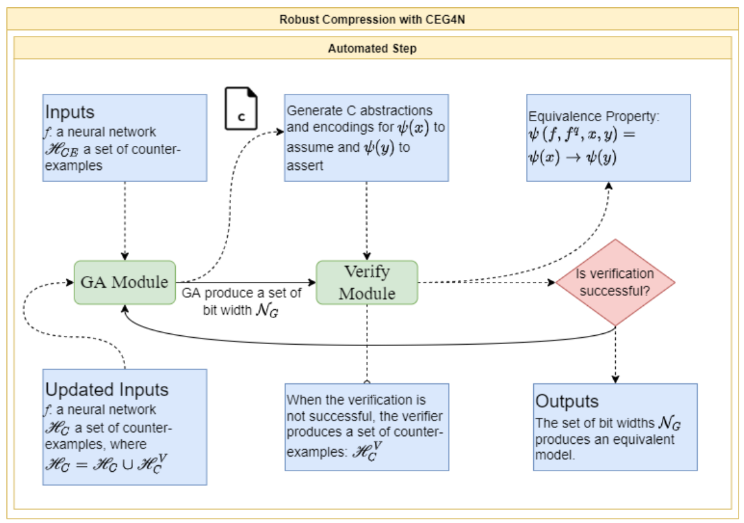
\includegraphics[width=0.8\linewidth]{framework.png} % Replace with your image file
    \caption{Diagram}
    \label{fig:image1}
  
\end{figure}

The CEG4N framework is divided into two main modules, based on the optimization and verification sub-problem. 

In the optimization sub-problem, we need to minimize the quantization bit widths, that is, finding a candidate set $N$ of parameters that will be used to quantize the ANN. Second, we need to verify the equivalence property, that is, checking if a NN quantized with the bit widths in $N$ is equivalent to the original NN. 

\begin{equation}
    N^o = \arg\min_{n_1,...,n_L} \sum_{l \in N_l <= L} n_l 
\end{equation}
    
$$
\begin{aligned}
& \arg\max f(x) = \arg\max f^q(x), & \forall x \in H^o_{CE} \\
& n_l \geq \underline{N} \vee n_l  \in N^o \\
& n_l  \leq \overline{N}  \vee n_l  \in N^o 
\end{aligned}
$$

In the Verification sub-problem $o$, we check whether the $N^o$ generated by the optimization sub-problem $o$ satisfies the following equivalence property:
\begin{equation}
\Psi(f,f^q, x,y)=\Psi_x(x)\rightarrow \Psi_y(y)
\end{equation}
if  $\Psi_x(x)\rightarrow \Psi_y(y)$ holds for the candidate $N^o$, the optimization halts and $N^o$ is declared as solution; otherwise, a new counter-example $H_{CE}$ is generated. Iteration o+1 starts where iteration o stopped. That is, the optimization sub-problem o + 1 receives as parameter a set of $H^{+1}_{CE}$ such that $H^{o+1}_{CE}=H^o_{CE}\cup x_{CE}$.

Supposing that the bottleneck of the CEG4N lies in the verification sub-problem, we have proposed to approach to improve the scalability. 


\begin{itemize}
    \item Find the most optimal SMT solver used by the ESBMC;
    \item Improve the Interval Analysis used by the ESBMC.
\end{itemize}
\section{Methodology}
\section{Result}
\section{Conclusion}

\subsection{}

%\section*{Acknowledgment}

%The preferred spelling of the word ``acknowledgment'' in America is without 
%an ``e'' after the ``g''. Avoid the stilted expression ``one of us (R. B. 
%G.) thanks $\ldots$''. Instead, try ``R. B. G. thanks$\ldots$''. Put sponsor 
%acknowledgments in the unnumbered footnote on the first page.

%\section*{References}

%Please number citations consecutively within brackets \cite{b1}. The 
%sentence punctuation follows the bracket \cite{b2}. Refer simply to the reference 
%number, as in \cite{b3}---do not use ``Ref. \cite{b3}'' or ``reference \cite{b3}'' except at 
%the beginning of a sentence: ``Reference \cite{b3} was the first $\ldots$''

%Number footnotes separately in superscripts. Place the actual footnote at 
%the bottom of the column in which it was cited. Do not put footnotes in the 
%abstract or reference list. Use letters for table footnotes.

%Unless there are six authors or more give all authors' names; do not use 
%``et al.''. Papers that have not been published, even if they have been 
%submitted for publication, should be cited as ``unpublished'' \cite{b4}. Papers 
%that have been accepted for publication should be cited as ``in press'' \cite{b5}. 
%Capitalize only the first word in a paper title, except for proper nouns and 
%element symbols.

%For papers published in translation journals, please give the English 
%citation first, followed by the original foreign-language citation \cite{b6}.

\begin{thebibliography}{00}
\bibitem{1} { João Batista P. Matos Jr and Iury Bessa and  Edoardo Manino and Xidan Song and Lucas C. Cordeiro, ``CEG4N: Counter-Example Guided Neural Network Quantization Refinement,''}

\bibitem{c2} {Bob Blumenscheid, Senior Product Marketing Manager, Digi International. "10 Real Life Examples of Embedded Systems." June 04, 2021. Available online: \url{https://www.digi.com/blog/post/examples-of-embedded-systems}}.

\bibitem{bnn_overview} R. Sayed, H. Azmi, H. Shawkey, A. H. Khalil, and M. Refky, ``A Systematic Literature Review on Binary Neural Networks,'' IEE Access, vol. 1, 2023.
\bibitem{c4} L. Sena, X. Song, E. Alves, I. Bessa, E. Manino, L. Cordeiro, and E. de Lima, ``Verifying Quantized Neural Networks using SMT-Based Model Checking,'' ACM Trans., vol. 1, 2021.
\bibitem{c5} Xidan Song, Youcheng Sun1, Mustafa
A. Mustafa, and Lucas C.
Cordeiro, ``QNNRepair: Quantized Neural Network Repair,'' ACM Trans., vol. 1, 2021.

\bibitem{c6} Luiz H. Sena, Xidan Song, Iury Bessa, Erickson Alves, Edoardo Manino, and Lucas C.
Cordeiro, ``Verifying Binarised Neural Networks using SMT-Based Model
Checking,'' Machester., vol. 1, 2022.

\bibitem{c7} Luiz H. Sena, Xidan Song, Iury Bessa, Erickson Alves, Edoardo Manino, Eddie De Lima Filho, and Lucas C.
Cordeiro, ``Verifying Quantized Neural Networks using SMT-Based
Model Checking'' Machester., vol. 1, 2022.

\bibitem{c8} Guy Amir, Haoze Wu, Clark Barrett, and Guy Katz , ``An SMT-Based Approach for Verifying
Binarized Neural Networks'' Machester., vol. 1, 2022.


%\bibitem{b3} I. S. Jacobs and C. P. Bean, ``Fine particles, thin films and exchange anisotropy,'' in Magnetism, vol. III, G. T. Rado and H. Suhl, Eds. New York: Academic, 1963, pp. 271--350.
%\bibitem{b4} K. Elissa, ``Title of paper if known,'' unpublished.
%\bibitem{b5} R. Nicole, ``Title of paper with only first word capitalized,'' J. Name Stand. Abbrev., in press.
%\bibitem{b6} Y. Yorozu, M. Hirano, K. Oka, and Y. Tagawa, ``Electron spectroscopy studies on magneto-optical media and plastic substrate interface,'' IEEE Transl. J. Magn. Japan, vol. 2, pp. 740--741, August 1987 [Digests 9th Annual Conf. Magnetics Japan, p. 301, 1982].
%\bibitem{b7} M. Young, The Technical Writer's Handbook. Mill Valley, CA: University Science, 1989.
\end{thebibliography}
%\vspace{12pt}
%\color{red}
%IEEE conference templates contain guidance text for composing and formatting conference papers. Please ensure that all template text is removed from your %conference paper prior to submission to the conference. Failure to remove the template text from your paper may result in your paper not being published.

\end{document}
